%%% Local Variables:
%%% mode: latex
%%% TeX-master: "../index"
%%% End:

% Recommended:
% Complexity of collisions (preimage)
% - Birthday paradox
% How to build hash functions
% - Blocks with padding
% - Merkle-Damgaard
% - Why is it secure?

\subsection*{Agenda}
\begin{enumerate}
\item Birthday paradox
\item Complexity of collisions
\item Iterated hash functions
\item Padding
\item Merkle-Damgård
\end{enumerate}
\subsection{Properties of Hash functions}

\textbf{Hash functions} takes a input of a binary string of arbitrary
length and returns a binary string of fixed length.
\begin{figure}[H]
  \centering
  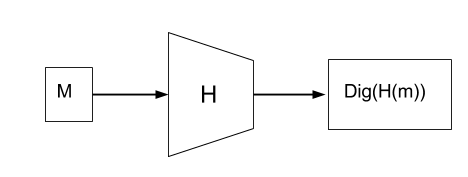
\includegraphics[scale=0.4]{images/10-hash}
  \caption{Model for hashing a message}
\end{figure}

\textbf{The ideal Hash function} has 4 main properties:
\begin{itemize}
\item [--]it is easy to compute the hash value for any given message
\item [--]it is infeasible to generate a message that has a given hash (pre-image)
\item [--]it is infeasible to modify a message without changing the hash
\item [--]it is infeasible to find two different messages with the same hash (collision)
\end{itemize}

\textbf{Security of Hash functions} 

% \textbf{Private key:}

% \textbf{Private key:}

\subsection{Birthday paradox}
Probability of finding a collision. Given a function $f$ that maps
values to $H$ different outputs, the probability of finding a
collision after $n$ randomly selected inputs is

\[ p(n; H) \approx 1 - e^{\frac{-n(n-1)}{2H}} \approx 1 - e^{\frac{-n^2}{2H}} \]

This expression can be invertedto $n(p; H)$ describing how many tries
$n$ it takes to reach a probability $p$ of collision

\[ n(p; H) \approx \sqrt{2H \ln \frac{1}{1 - p}} \]

To achieve $0.5$ chance of collision this gives

\[ n(0.5; H) = 1.1774 \sqrt{H} \]

\textbf{Example:} For a 128 bit hash there are $2^{128}$ different
hashes, and the number of tries needed to achieve $0.5$ chance of
collision is then

\[ 1.1774 \sqrt{2^{128}} \approx 2.17 \cdot 10^{19} \]

\subsection{Iterated Hash functions}


\subsection{Padding}
\begin{figure}[H]
  \centering
  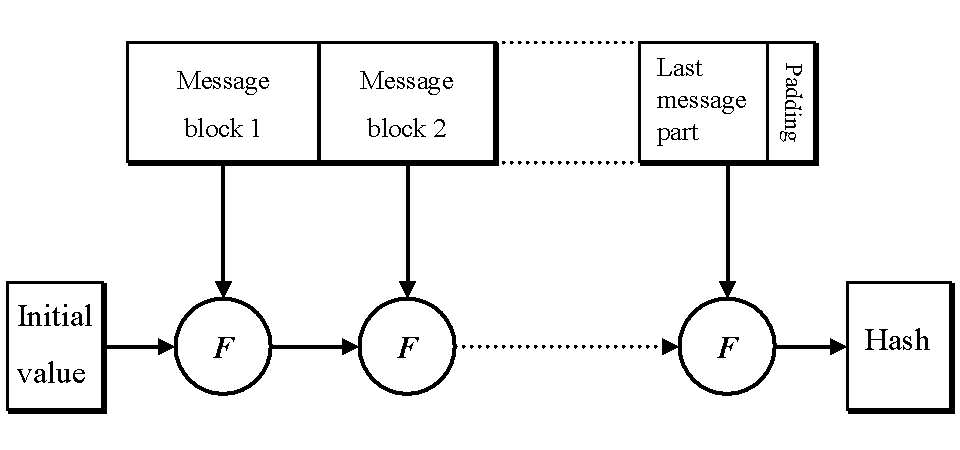
\includegraphics[scale=0.3]{images/10-padding}
  \caption{Model for hashing using padding}
\end{figure}

\subsection{Merkel-Damgård}
